
% PACKAGES INCLUDED HERE 
% DO NOT NEED TO CHANGE
\documentclass[conference]{IEEEtran}
%\IEEEoverridecommandlockouts
% The preceding line is only needed to identify funding in the first footnote. If that is unneeded, please comment it out.
\usepackage{cite}
\usepackage{amsmath,amssymb,amsfonts}
\usepackage{algorithmic}
\usepackage{graphicx}
\usepackage{textcomp}
\def\BibTeX{{\rm B\kern-.05em{\sc i\kern-.025em b}\kern-.08em
    T\kern-.1667em\lower.7ex\hbox{E}\kern-.125emX}}
\begin{document}

% TITLE GOES HERE

\title{Paper Title*\\}


% AUTHOR NAMES GOES HERE

\author{\IEEEauthorblockN{1\textsuperscript{st} Given Name Surname}
\IEEEauthorblockA{\textit{dept. name of organization (of Aff.)} \\
\textit{name of organization (of Aff.)}\\
City, Country \\
email address}
\and
\IEEEauthorblockN{2\textsuperscript{nd} Given Name Surname}
\IEEEauthorblockA{\textit{dept. name of organization (of Aff.)} \\
\textit{name of organization (of Aff.)}\\
City, Country \\
email address}
\and
\IEEEauthorblockN{3\textsuperscript{rd} Given Name Surname}
\IEEEauthorblockA{\textit{dept. name of organization (of Aff.)} \\
\textit{name of organization (of Aff.)}\\
City, Country \\
email address}
\and
\IEEEauthorblockN{4\textsuperscript{th} Given Name Surname}
\IEEEauthorblockA{\textit{dept. name of organization (of Aff.)} \\
\textit{name of organization (of Aff.)}\\
City, Country \\
email address}
\and
\IEEEauthorblockN{5\textsuperscript{th} Given Name Surname}
\IEEEauthorblockA{\textit{dept. name of organization (of Aff.)} \\
\textit{name of organization (of Aff.)}\\
City, Country \\
email address}
\and
\IEEEauthorblockN{6\textsuperscript{th} Given Name Surname}
\IEEEauthorblockA{\textit{dept. name of organization (of Aff.)} \\
\textit{name of organization (of Aff.)}\\
City, Country \\
email address}
}

\maketitle

% ABSTRACT 

\begin{abstract}
This document is a model and instructions for \LaTeX.
This and the IEEEtran.cls file define the components of your paper [title, text, heads, etc.]. *CRITICAL: Do Not Use Symbols, Special Characters, Footnotes, 
or Math in Paper Title or Abstract.
\end{abstract}


% KEYWORDS

\begin{IEEEkeywords}
component, formatting, style, styling, insert
\end{IEEEkeywords}

% INTRODUCTION SECTION
\section{Introduction}

It is said that our children are our future, and for that reason we, as a society, try our best to prepare them for the world they live. Secondary education helps accomplish this by bridging the gap from primary education to either post-secondary, vocational training, or the work force. Whichever path an individual decides to take, secondary education is crucial for the prosperity of a nation. With secondary education related to unemployment and incarceration rates, the importance of education becomes apparent to a society \cite{mitra}. The United States addresses this by spending 5.62\% of its GDP on education -- this equals more than a trillion dollars \cite{nationmaster}. However, many students still fall short of finishing a post-secondary education. Yearly, over 1.2 million individuals in high school dropout in the United States \cite{miller2011}. Can we assume that there are certain contributing factors to a student's success in a secondary institution? And if we can, how do we identify what they are?  Using a neural network, this is what we intend to find out. 

% BACKGROUND SECTION
\section{Background}

Research in student performance has been aided many times using neural networks. Researchers at the University of Technology Mara Malaysia used a neural network to determine which early subjects in electrical engineering contributed the most towards the student’s success in the major. Data on 391 students was collected from the university. The input data consisted of student grades for individual subjects (six subjects per student) in an early semester while the output is predicting the cumulative grade point average. Using sigmoid for the hidden layer, purelin for the outer layer, they were able to achieve a relatively low Mean Squared Error (0.05544) \cite{arsad2013}. However, this neural network is limited in that it only considers quantitative data. 

 In the European Union, Portugal ranks the lowest with student success rates. Paulo Cortez and Alice Silva, Information Systems Scientists at the University of Minho in Portugal, collected data on the secondary public-school system to see if a neural network could determine factors contributing to the high failure rates of their youth. In their study, 788 students were given questionnaires with predefined options. Along with the questionnaires, past exam grades and attendance were collected; 139 samples were discarded due to faulty sampling leaving 649 confident samples. Using a feed-forward classification neural network, they were able to achieve 72\% accuracy with three classes and 62\% accuracy with nine classes \cite{cortez2008}. This study considered both qualitative and quantitative data which is why we use the same sample collected for our neural network. 

% METHODS SECTION
\section{Methods}

Our data consists of information concerning students from two schools in Portugal during the 2005-2006 school year. Information was collected both from school results along with questionnaires, which are used to determine additional details about the students’ environments. We are interested in grade information, which is scored on a scale of 0-20, along with other information about the students’ environment. Some of the information includes parental education, alcohol consumption, health status, and past class failures. We looked at student performance in Portuguese of which there are 649 records. 

With some of our input data being qualitative, we had to encode it for the network. This was done by using a label encoder tool provided by Scikit-learn. This was done for all binomial and nominal data. Zeros (0) were encoded to negative ones (-1) for the binomial data to ensure proper weight updates. In addition, we needed to shuffle our dataset due to its ordered nature. Without this step, we would be training on data exclusively from one school, then testing on data from a different school. 

For our network’s output shape, we decided to attempt classification of student’s scores into 5 categories. The categories range from 0, the worst score, to 4. We use a keras sequential model with two hidden layers for our simple feed-forward network. Both of these layers have the rectified linear unit as its activation function. ReLU is used because it avoids activations of zero, which can be an issue with softmax, while still allowing for nonlinearity. The function is defined as $f(x) = max(0,x)$ \cite{kaggle}. An image of the function is shown in Figure \ref{relu}.

\begin{figure}[htbp]
\centerline{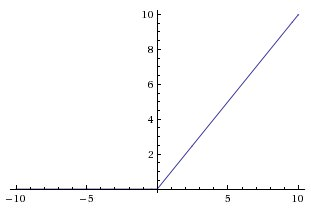
\includegraphics[width=\linewidth]{relu.jpg}}
\caption{A graph showing the form of ReLU \cite{kaggle}.}
\label{relu}
\end{figure}

The first hidden layer has 800 units while the second has 400. The final, output layer uses the softmax activation function, which allows us to predict one of several categories. The error function we selected is categorical cross entropy due to its ability to help us classify students into one of multiple different categories. 

Now that we have a network which we believe can predict student scores, we split our data into two sets, one for training and one for testing of the trained network. After several trials, we decided that beyond 7 epochs, our model began overfitting, so we stopped at that point. As our main objective is determining what factors contribute the most to student success, after an initial test, we began testing the network while removing a single feature every trial. Afterwards, we attempted to determine which features had the greatest impact on our model’s performance. We then selected the most detrimental of those features and removed them all at the same time, hoping to improve our results.

% RESULTS SECTION
\section{Results}

During the initial test of the network, a test accuracy of 77\% was achieved while using all features in the data set. It was thought that this accuracy could be increased by removing redundant features. This test is depicted in figure \ref{results1}

\begin{figure}[htbp]
\centerline{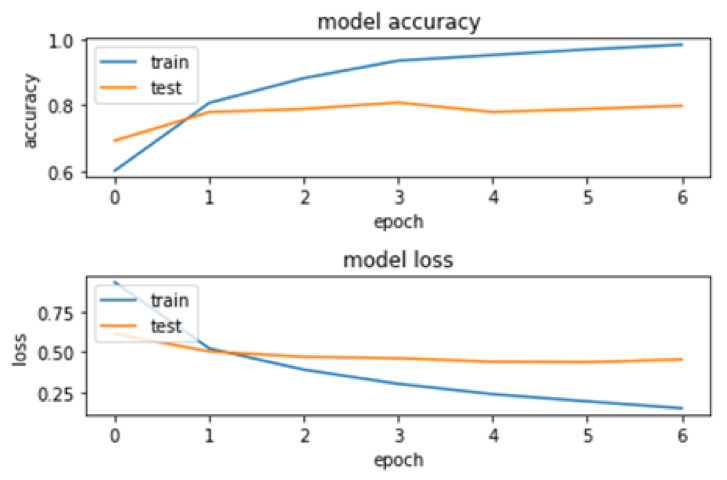
\includegraphics[width=\linewidth]{results1.png}}
\caption{Initial test results.}
\label{results1}
\end{figure}

There were two features whose removal from the training data had little effect on the network’s accuracy. The removal of the school and grade three features saw little to no increase in network accuracy. Figure \ref{results2} is from the network that trained on the data without the grade three feature.

\begin{figure}[htbp]
\centerline{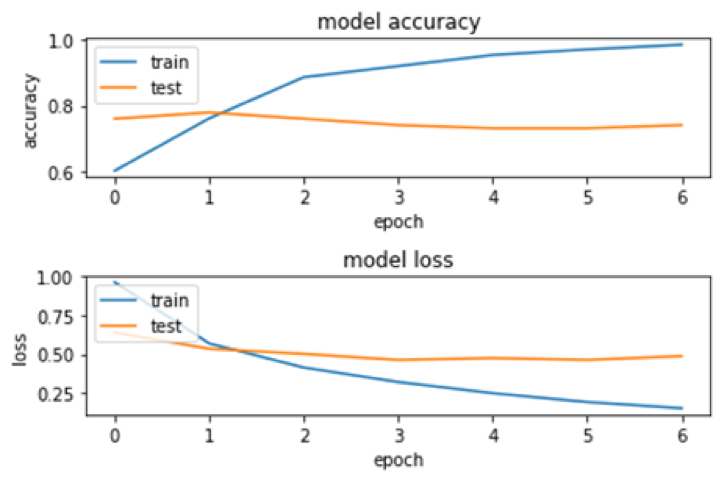
\includegraphics[width=\linewidth]{results2.png}}
\caption{Test results without grade 3.}
\label{results2}
\end{figure}

Aside from the two features listed above, the removal of any other feature from the data set caused the network’s test accuracy to increase significantly. The removal of the feature that describe the mother’s occupation caused the test accuracy to increase to 88\%. The same is true for the feature that describes the number of absences the student has, and the higher education feature. Figure \ref{results3} depicts network accuracy and loss with the absence feature removed.

\begin{figure}[htbp]
\centerline{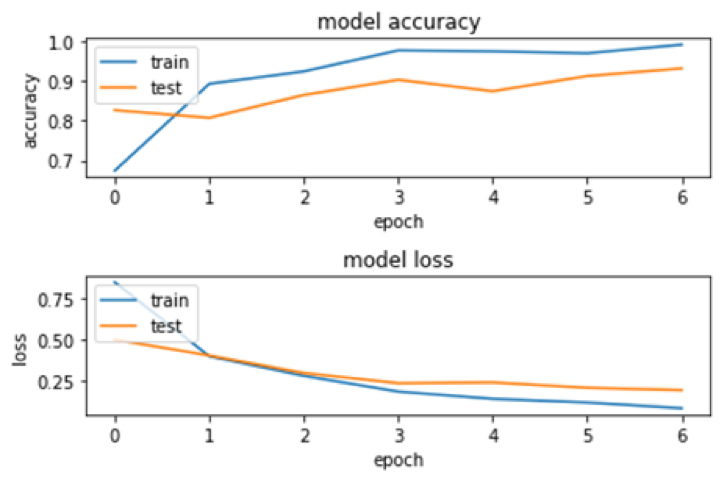
\includegraphics[width=\linewidth]{results3.png}}
\caption{Test results without absences.}
\label{results3}
\end{figure}

The highest test accuracy achieved was 97\% accuracy. This accuracy rating was reached on three different occasions of feature removal: the removal of the age feature, the removal of the address feature, and the removal of the free time feature. Figure \ref{results4} depicts the overall accuracy and loss of the network after the removal of the age feature.

\begin{figure}[htbp]
\centerline{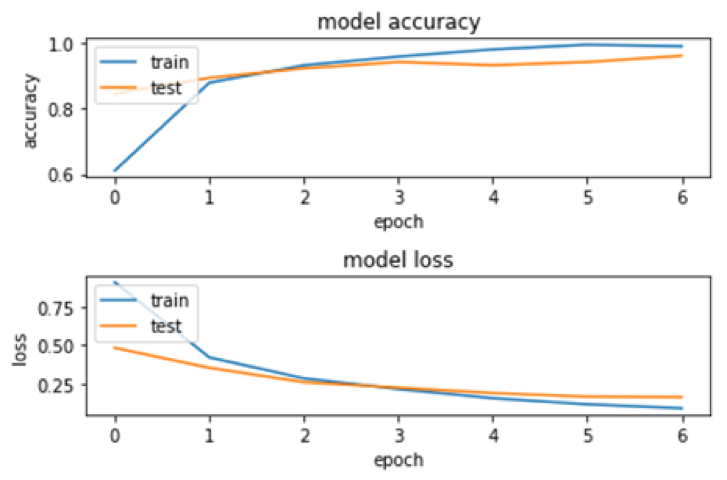
\includegraphics[width=\linewidth]{results4.png}}
\caption{Test results without age.}
\label{results4}
\end{figure}

The removal of other features from the training set generally resulted in a test accuracy between 90\% and 97\%. The highest accuracy among this group is 96\%, after the removal of the feature that described how much alcohol a student drank on the weekend. A test accuracy of 90\% was the lowest accuracy score of this group, after the removal of the travel time feature from the training set. Figure \ref{results5} shows the accuracy and loss of the network that was trained without the travel time feature.

\begin{figure}[htbp]
\centerline{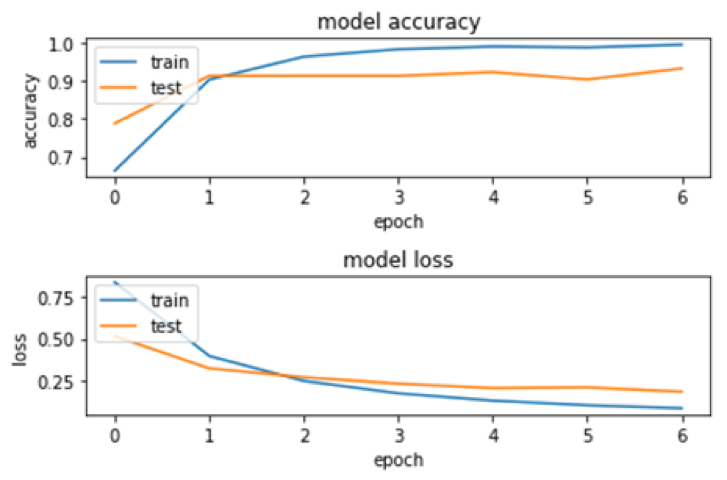
\includegraphics[width=\linewidth]{results5.png}}
\caption{Test results without travel time.}
\label{results5}
\end{figure}

Other notable features are the grade one and grade two feature, whose removal saw an increase in test accuracy to 90\% and 93\% respectively. Features like internet access and romantic involvement, after removal, saw a test accuracy of 95% and 96% respectively.

% DISCUSSION SECTION
\section{Discussion}

Start typing here \cite{b5}.

% REFERENCES
% THIS IS CREATED AUTOMATICALLY
\bibliographystyle{IEEEtran}
\bibliography{References} % change if another name is used for References file

\end{document}
